\documentclass[11pt]{jarticle}
\usepackage{graphicx}
\begin{document}
方程式$f(x)=0$の{\em 解}とは,関数$f(x^*)=0$を満たす$x^*$のことを言う.図\ref{figure}では,曲線$y=f(x)$と$x$軸が交わっており,この交点の$x$座標が$x^*$である.

 いま,解$x^*$の近似値$x_k$が与えられているとする.点$(x_k,f(x_k))$における曲線$y=f(x)$の接線(図中の斜めの線)の方程式は$y=f(x_k)+(x-x_k)・f'(x_k)$である.ここで,$f'(x)$は$f(x)$の導関数である.この接線と$x$軸の交点$(x_{k+1})$は次の式で表される\cite{text2017}.
\begin{equation}
x_{k+1}=x_k-\frac{f(x_k)}{f'(x_k)}
\label{eq:intersection}
\end{equation}
図1の場合,$x_{k+1}$が$x_k$よりも解$x^*$に近い.このため,適当な初期値$x_0$を与え,式(\ref{eq:intersection})によって数列($x_k$)を定義すると,この数列は$k \rightarrow \infty $で$x^*$に{\em 収束}することが期待される.
\begin{figure}[h]
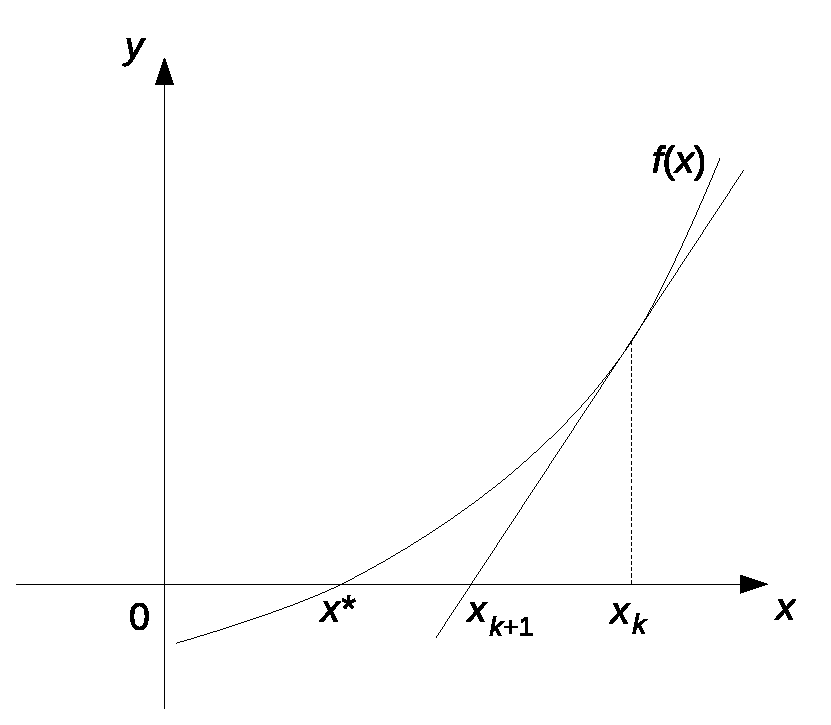
\includegraphics{p1/old/figure2.eps}
\caption{ニュートン法の原理}
\label{figure}
\end{figure}
\begin{thebibliography}{99}
\bibitem{text2016} 著者1, 著者2, 「書名1」, 出版社1, pp.ページ範囲,(2014).
\bibitem{text2017} 著者3, 「書名2」, 出版社2, pp.ページ範囲,(2019).
\end{thebibliography}
\end{document}
